\documentclass[border=50pt]{standalone}
\usepackage{tikz}

% Calculate the circle radius based on mass
\newcommand{\calculateRadius}[1]{sqrt(#1/3.14159)}

\begin{document}
% \fbox{
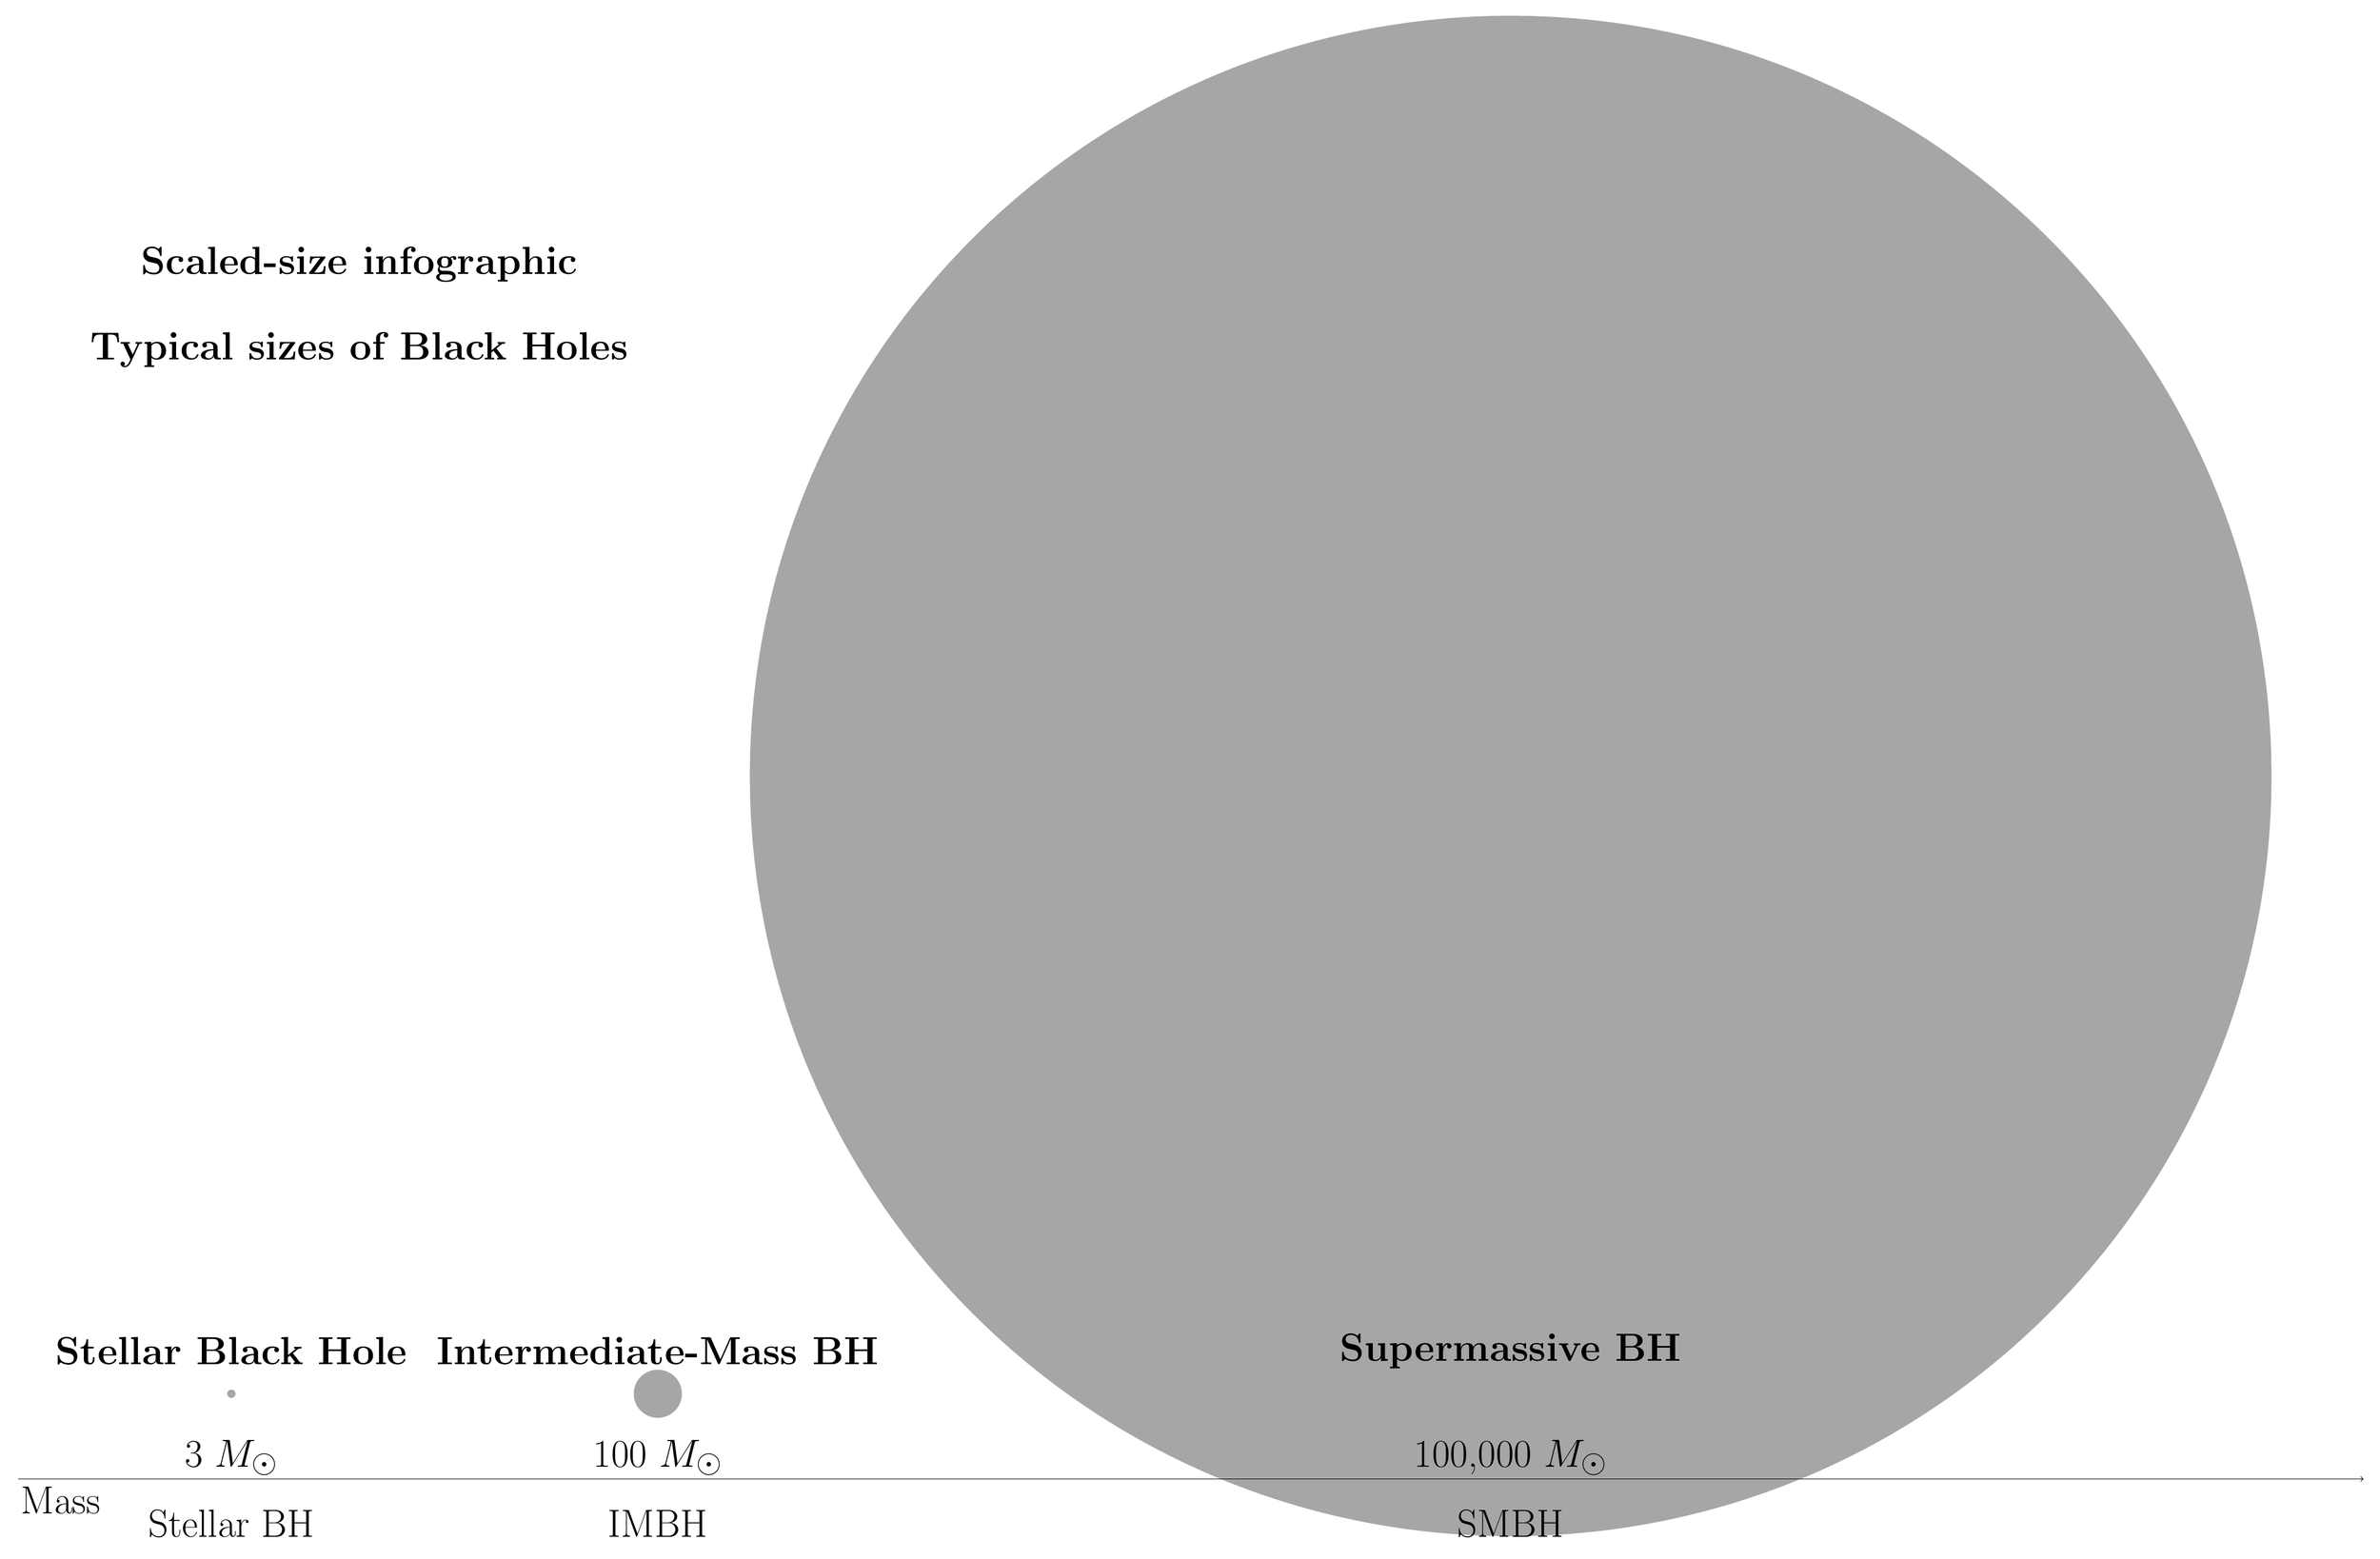
\begin{tikzpicture}[scale=0.95]
  % Stellar Black Hole
  \pgfmathsetmacro{\stellarBHmass}{0.03}
  \pgfmathsetmacro{\stellarBHradius}{\calculateRadius{\stellarBHmass}}
  \fill[gray!70] (0,-14.5) circle (\stellarBHradius cm);
  \node[black] at (0,-13.5) {\textbf{\Huge{Stellar Black Hole}}};

  % Intermediate-Mass Black Hole
  \pgfmathsetmacro{\IMBHmass}{1}
  \pgfmathsetmacro{\IMBHradius}{\calculateRadius{\IMBHmass}}
  \fill[gray!70] (10,-14.5) circle (\IMBHradius cm);
  \node[black] at (10,-13.5) {\textbf{\Huge{Intermediate-Mass BH}}};


  % Supermassive Black Hole
  \pgfmathsetmacro{\SMBHmass}{1000}
  \pgfmathsetmacro{\SMBHradius}{\calculateRadius{\SMBHmass}}
  \fill[gray!70] (30,0) circle (\SMBHradius cm);
  \node[black] at (30,-13.5) {\textbf{\Huge{Supermassive BH}}};


  % Mass Scale
  \draw[->] (-5,-16.5) -- (50,-16.5);
  \node at (-4,-17) {\Huge{Mass}};
  \foreach \x/\text in {0/\Huge{Stellar BH}, 10/\Huge{IMBH}, 30/\Huge{SMBH}} {
    \draw (\x,-18) -- (\x,-18) node[above] {\text};
  }
  \node at (0,-16) {\Huge{3 $M_{\odot}$}};
  \node at (10,-16) {\Huge{100 $M_{\odot}$}};
  \node at (30,-16) {\Huge{100,000 $M_{\odot}$}};
  \node at (3, 12) {\Huge{\textbf{Scaled-size infographic}}};
  \node at (3, 10) {\Huge{\textbf{Typical sizes of Black Holes}}};
\end{tikzpicture}
% }
\end{document}
